%=========================================================
\chapter{Propuesta}
\label{cap:Propuesta}
El \textbf{Instituto Mexicano del Seguro Social} es una institución cuya misión es ser el instrumento básico de la seguridad social, establecido como un servicio público de carácter nacional, para todos los trabajadores y trabajadoras y sus familias.\\

El instituto actualmente maneja su información por medio de archivos de excel, debido a este constante intercambio de actualización de información es por lo que la empresa requiere un sistema que se adapte y este diseñado para cubrir cada una de las necesidades en la operación interna del instituto.

\section{Análisis del problema}

\subsection{Problema general}
El problema general de la empresa recae en la desorganización en la información que se ha vuelto inconsistente por falta de actualización constante, impactando directamente a otras áreas que hacen uso de la información referente a los empleados.

\subsection{Problemas específicos}
La información actualmente se maneja mediante archivos de excel, al no manejar la información de manera eficiente en la que los empleados puedan obtener la información lo más pronto posible, tener la información actualizada y visible para todos, ha generado los siguientes problemas:

\begin{enumerate}
    \item Desactualización del correo de contacto de los empleados.
    \item Retardo en tiempos para contactar a los empleados de las distintas Delegaciones y UMAES.
    \item Desactualización del número telefónico de contacto de los empleados.
\end{enumerate}

\subsection{Causas}
Las principales causas se deben a que actualmente no se cuenta con un correcto control en la realización de las siguientes actividades:
\begin{enumerate}
    \item Solicitud de cambios de información de los empleados.
    \item Actualización de información de los empleados.
\end{enumerate}

\subsection{Consecuencias}
Como consecuencias dentro de la institución:
\begin{itemize}
    \item Envío de información hacia correos equivocados.
    \item Llamadas a números equivocados.
\end{itemize}

\subsection{Requerimientos de usuario}
\newcommand{\RUitem}[5]{\par{#1} & {#2} & {#3}\\ \hline}
\begin{longtable}{|p{.1\textwidth}|p{.2\textwidth}|p{.6\textwidth}|}
  \hline 
  \RUitem{\textbf{ID}}{\textbf{Nombre}}{\textbf{Descripción}} \\ \hline
  \endfirsthead

  \multicolumn{3}{c}%
  {{\bfseries \tablename\ \thetable{} Continuación de la página anterior}} \\
  \hline 
  \RUitem{\textbf{ID}}{\textbf{Nombre}}{\textbf{Descripción}} \\ \hline
  \endhead

  \hline \multicolumn{3}{|l|}{{Continúa en la siguiente página}} \\ \hline
  \endfoot
  \hline \hline
  \endlastfoot%
  %Agregar aquí lo requerimientos de usuario
    \RUitem{\hypertarget{ReqUsr:RU-1}{RU-1}}{Inicio de sesión}{Todo empleado necesita una herramienta que le permita acceder al sistema.} \\ \hline
    
    \RUitem{\hypertarget{ReqUsr:RU-2}{RU-2}}{Cierra de sesión}{Todo empleado necesita una herramienta que le permita salir del sistema.} \\ \hline
  
    \RUitem{\hypertarget{ReqUsr:RUADM-1}{RUADM-1}}{Herramienta de alta}{El administrador necesita una herramienta que lo auxilie para agregar la información de los empleados en las distintas UMAES y Delegaciones.} \\ \hline

    \RUitem{\hypertarget{ReqUsr:RUADM-2}{RUADM-2}}{Herramienta de cambios}{El administrador necesita una herramienta que lo auxilie para modificar la información de los empleados en las distintas UMAES y Delegaciones.} \\ \hline 

    \RUitem{\hypertarget{ReqUsr:RUADM-2}{RUADM-2}}{Herramienta de bajas}{El administrador necesita una herramienta que lo auxilie para eliminar la información de los empleados en las distintas UMAES y Delegaciones.} \\ \hline 

    \RUitem{\hypertarget{ReqUsr:RUCS-1}{RUCS-1}}{Herramienta de consulta}{El consultor necesita una herramienta que lo auxilie para conocer la información de los empleados en las distintas UMAES y Delegaciones.} \\ \hline

    \RUitem{\hypertarget{ReqUsr:RUED-1}{RUED-1}}{Herramienta de cambios}{El administrador necesita una herramienta que lo auxilie para modificar la información de los empleados en las distintas UMAES y Delegaciones.} \\ \hline 

\end{longtable}
\section{Propuesta de solución}
Con el fin de resolver los problemas anteriormente mencionados que enfrenta el IMSS, propone la creación de un software que permita mejorar y optimizar su funcionamiento haciendo que las distintas actividades que realizan los empleados día con día como son : El envío de correos, realización de llamadas, entre otras puedan ser llevadas a cabo de una manera más fácil, de forma organizada y eficiente.

\subsection{Objetivos generales}
Desarrollar un software para el IMSS que le permita tener un mayor control, organización e información relacionada con los empleados de las distintas Delegaciones y UMAES, así como mejorar la comunicación con los distintos departamentos para una centralización de los datos respecto a empleados, asimismo para evitar la pérdida de información y manteniéndola actualizada.

\subsection{Objetivos específicos}

\begin{itemize}
    \item Dar de alta a los nuevos empleados.
    \item Conocer la información de los empleados o de un sólo empleado de manera concreta.
    \item Modificar la información de algún empleado en específico.
    \item Dar de baja a empleados que ya no laboran dentro del instituto.
\end{itemize}

\subsection{Descripción de la solución}
Se propone un sistema el cuál contará con las siguientes características:\\
El \hyperlink{UsrDef:Administrador}{Administrador} podrá:
\begin{itemize}
	\item Tener una cuenta para acceder al sistema. 
	\item Dar de alta a nuevos empleados al directorio.
	\item Modificar la información de los empleados en caso de que sea necesario.
	\item Eliminar a un empleado en caso de que este ya no trabajé más para el instituto.
	\\
\end{itemize}

El \hyperlink{UsrDef:Consultor}{Consultor} podrá:
\begin{itemize}
	\item Visualizar la información de 
    \\
\end{itemize}

El sistema propuesto buscará concentrar la información de los empleados de una forma ordenada, facilitando a los demás empleados el acceso a la información de su interés. Beneficiando así la realización de las siguientes tareas:
\begin{itemize}
    \item Evitará la inconsistencia de información perteneciente a los empleados, como era el caso de el envío de información de un empleado laborando en el instituto a otro que dejó de laborar en el instituto.
\end{itemize}
\section{Alcance}

\subsection{Requerimientos funcionales}

\begin{enumerate}[leftmargin=2.5cm ,label={\bfseries RF-\arabic*}]
  
    % Permisos
    \item \textbf{Inicio de sesión:} El sistema debe de contar con un inicio de sesión para los distintos roles. Sólo los usuarios autorizados de esta forma podrán acceder a los datos del sistema.
    \textbf{Ref:} \hyperlink{ReqUsr:RU-1}{RU-1}
    \textbf{Prioridad:}MA

    \textbf{Alta de empleados:} El sistema debe de contar con un módulo de alta de empleados. Sólo los usuarios autorizados podrán darlos de alta en el sistema.
    \textbf{Ref:} \hyperlink{ReqUsr:RUADM-1}{RUADM-1}
    \textbf{Prioridad:}A

    \textbf{Modificación de información de empleados:} El sistema debe de contar con un módulo para la modificación de información de empleados. Sólo los usuarios autorizados podrán modificar su información dentro del sistema.
    \textbf{Ref:} \hyperlink{ReqUsr:RUADM-2}{RUADM-2}, \hyperlink{ReqUsr:RUED-1}{RUED-1}
    \textbf{Prioridad:}A
    
    \textbf{Consulta de información de empleados:} El sistema debe de contar con un módulo para la modificación de información de los empleados. Sólo los usuarios autorizados podrán consultar la información de los empleados en el sistema.
    \textbf{Ref:} \hyperlink{ReqUsr:RUCS-1}{RUCS-1}
    \textbf{Prioridad:}M
    
    \textbf{Baja de empleados:} El sistema debe de contar con un módulo para dar de baja a los empleados que ya no laboran más dentro del instituto. Sólo los usuarios autorizados podrás realizar está acción dentro del sistema.
    \textbf{Ref:} \hyperlink{ReqUsr:RUADM-2}{RUADM-2}
    \textbf{Prioridad:}M

    \item \textbf{Cierre de sesión:} El sistema debe de contar con un cierre de sesión para los distintos roles. Todos los usuarios autorizados de esta forma podrán cerrar su sesión en el sistema.
    \textbf{Ref:} \hyperlink{ReqUsr:RU-2}{RU-2}
    \textbf{Prioridad:}MA

\end{enumerate}%ya incluye 3.3Alcance
\subsection{Requerimientos no funcionales}

\subsubsection{Plataforma}
La plataforma del sistema sera bajo la arquitectura cliente - servidor, puesto que es una pagina web la cual accederá a
un servidor para realizar las operaciones de consulta, agregación y eliminación de datos.

%\begin{figure}[htbp!]
%	\begin{center}
%		\fbox{\includegraphics[width=\textwidth]{proc/Dibujo.jpg}}
%		\caption{Arquitectura del sistema.}
%		\label{fig:arquitectur}
%	\end{center}
%\end{figure}


\begin{itemize}


    \item Visualización en los navegadores más comunes como son Edge, Firefox y Chrome.
    \item Se utilizará el gestor de base de datos PostgreSQL.
\end{itemize}

\textbf{Especificaciones del servidor}
\begin{itemize}
 \item XX GB  de memoria RAM
 \item XX GB de disco duro
 \item Sistema Operativo XXXXXXXX

 \item Apache/2.4.18
 \item PHP Version: 5.6
 \item PostgreSQL 9.2 o 9.4
\end{itemize}
\textbf{Especificaciones de la computadora del cliente}
\begin{itemize}
\item Windows 7, Windows 8, Windows 8.1, Windows 10 o superior
\item Intel Pentium 4 o superior
\item Linux 64-bit Ubuntu 14.04+, Debian 8+, openSUSE 13.3+, o Fedora Linux 24+
\item Intel Pentium 4 o superior
\item Memoria Ram: 2GB o superior
\end{itemize}%ya incluye 3.3.2Requerimientos no funcionales
\hypertarget{cap:infoydats}{}
\subsubsection{Información y datos}
\textbf{Modelo de dominio - Delegación}
Dentro del siguiente modelo de datos se presenta un prototipo en modelo Entidad-Relación de la delegación.

\begin{figure}[htbp!]
	\begin{center}
	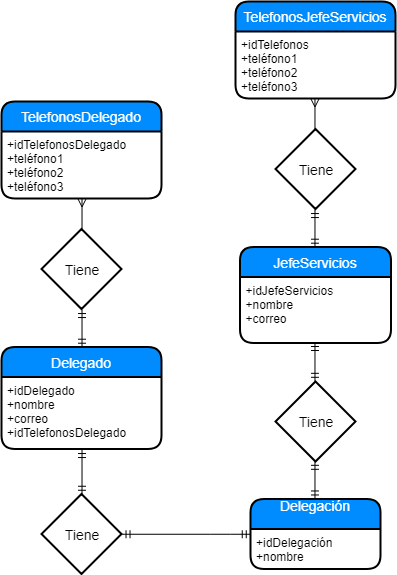
\includegraphics[width=.60\textwidth]{images/capitulo3/ModeloDominio.png}
		\caption{Modelo de dominio de programa}
		\label{InfoyDatos:ModeloDominio}
	\end{center}
\end{figure}
\clearpage